\documentclass[12pt]{report}
\usepackage{djtex}
\usepackage{titlesec}
\usepackage{color}
\usepackage{enumitem}
\usepackage{caption}

\setcounter{secnumdepth}{3}

% Remove all the excessive space from the chapter headers.
\titleformat{\chapter}[display]   
{\normalfont\huge\bfseries}{\chaptertitlename\ \thechapter}{20pt}{\Huge}   
\titlespacing*{\chapter}{0pt}{-50pt}{40pt}
% End chapter header fix.

\newenvironment{reqlist}{
	\renewcommand{\labelenumi}{\tab\thesubsection.\arabic{enumi}}
	\renewcommand{\labelenumii}{\thesubsection.\arabic{enumi}.\arabic{enumii}}
	\begin{enumerate}[itemsep = 1pt, parsep = 0pt, leftmargin = *]
}{\end{enumerate}}

% Remove chapter number from sections.
\renewcommand*\thesection{\arabic{section}}

\begin{document}

% Create Header.
\header{Capstone Requirements Specification}{}{Group 4}

\captionsetup[figure]{font=scriptsize, labelfont={bf},skip=0pt}

% Create Title Page.
\font\titlefont = cmr12 at 50pt
\font\subtitlefont = cmr12 at 28pt
\title{\titlefont{Capstone Project} \\ \vspace{10pt} \subtitlefont{Software Requirements Specification}}
\author{Roberto E. Acevedo Morales \\ Adrian Gonzalez \\ Dan Jones \\ Rajat Singh}
\date{}
\maketitle

\tableofcontents \newpage

\section{Introduction}
	\subsection{Purpose: Mission Statement}
		The goal of our team was to bring the excitement and uncertainty of distant galaxies to a browser window with a fast-paced arcade style game containing infinitely generating obstacles, enemies, and adventure.
	\subsection{Scope}
		The capstone project completed by Group 4, herein referred to as ``The System,'' shall consist software, audio, and graphical assets combined to provide an entertaining gaming experience harkening back to traditional arcade titles such as Galaga and Space Invaders, but with some modern twists.
	\subsection{Definitions, Acronyms, and Abbreviations}
		\begin{reqlist}
			\item \textbf{Application Programming Interface (API)} \\ A set of commands, functions, protocols, and objects that programmers can use to create software or interact with an external system.
			\item \textbf{Directional Keys} \\ Keys on a user's keyboard including the arrow keys or ``WASD" keys that are used for basic player movement.
			\item \textbf{Frame Rate} \\ The rate at which consecutive images called ``frames" are displayed while rendering film or computer graphics.
			\item \textbf{Game Engine} \\ A framework for game development that provides inherent support for various common components of a game such as physics, animation, audio, and lighting.
			\item \textbf{Graphical User Interface (GUI)} \\ A user interface that includes graphical elements, such as windows, icons and buttons. Interactions with the GUI are typically completed with a mouse and keyboard.
			\item \textbf{HTML5} \\ A W3C specification that defines the fifth major revision of the Hypertext Markup Language (HTML).
			\item \textbf{Leaderboard} \\ A table displaying the names of users with the top-10 highest scores in the game.
			\item \textbf{Pickup} \\ Any generated item that can be collected by the user by colliding with it. They offer positive effects for the player such as replenishing health or energy or adding to the user's in-game currency.
			\item \textbf{Player} \\ The virtual protagonist in the game which is controlled by the user during gameplay. This is differentiated from the ``user" role in this document.
			\item \textbf{Round} \\ One round of gameplay consists of the time they are able to control the player until exhausting all of the player's lives.
			\item \textbf{Score} \\ Within the context of The System, the uesr's score is determined by the amount of time they were able to survive during a single round of gameplay.
			\item \textbf{Session} \\ The timeframe between when the user first launches The System and when they exit The System.
			\item \textbf{Side Scroller} \\ A type of game in which a side-view camera angle is used to view a character travelling from left to right on the screen, involving movement in one continuous direction in many cases.
			\item \textbf{Terrain} \\ A combination of randomly generated obstacles and enemies that make up the game world through which the user must navigate in order to survive for the longest time possible.
			\item \textbf{User} \\ The human individual interacting with The System. This is differentiated from the ``player" role in this document.
			\item \textbf{User Interface (UI)} \\ See ``Graphical User Interface (GUI)." The terms may be used interchangeably in this document.
			\item \textbf{WebGL} \\ A JavaScript API for rendering interactive 2D and 3D graphics within any compatible web browser without the use of plug-ins.
			\item \textbf{World Wide Web Consortium (W3C)} \\ An international community where Member organizations, a full-time staff, and the public work together to develop web standards. 
		\end{reqlist}
	\subsection{References}
		\begin{reqlist}
			\small{
				\item https://techterms.com/definition/api
				\item https://en.wikipedia.org/wiki/Frame\_rate
				\item https://unity3d.com/what-is-a-game-engine
				\item https://techterms.com/definition/gui
				\item https://www.techopedia.com/definition/27153/side-scroller
				\item https://www.webopedia.com/TERM/H/HTML5.html
				\item https://www.w3.org/Consortium/
			}
		\end{reqlist}
	\subsection{Overview}
		The following document outlines the software requirements and specificatiosn for The System, including the fucntional, nonfunctional, domain, hazard, and system requirements. Requirements are organized into sections based on their applicability to more general goals such as resources used on the player's end, the features incorporated within the game, and how the game performs under appropriate conditions.

\section{Overall Description}
	This section is intended to provide an overview of The System as a whole. It will explain the basic functionality of The System and how its various components interact with each other. It will also provide some insight regarding potential users and stakeholders, and list the constraints and dependencies involved in the development and use of The System.
	\subsection{Product Perspective}
		The system consists of a variety of different software modules, auditory, and visual assets all packaged within a singular final build. It can be hosted on an HTTP server to be accessed by any user with a link. Accessing and interacting with the system will all be performed within the web browser chosen by the user. Support for different browsers and adherence to web-based standards and protocols is left up to the build process supplied by the Unity Game Engine.
	\subsection{Product Functions}
		The functions of The System are divided into two major categories: gameplay and navigation. The gameplay category can be further subdivided into three additional subcategories: movement, offense, and collection. The movement subcategory involves using the directional keys to navigate through the randomly generated terrain. Movement can be used for defensive purposes to avoid obstacles or to position the player for an attack. The offense subcategory involves using the mouse to rotate the player and firing at obstacles or enemies. This can be done for the purpose of eliminating threats from enemies, or clearing up the terrain for safer movement. The collection subcategory involves the user strategically selecting randomly generated pickups to collect in order to recover health and energy, as well as add to their in-game currency.
\\ \\
The navigation category includes any interactions the user carries out with the various features present in the UI included with the game. Such interactions mainly take place outside of the gameplay -- before the user has begun playing or after the player has died. Once The System is launched, the user is greeted with a main menu which provides them with control over when the gameplay begins. This main menu contains a settings page which allows the user to adjust their volume settings or delete their progress and other saved data. Upon exhausting all the player's lives during gameplay, a ``game over" screen is displayed to the user. This provides them with four options: return to the main menu, begin another round of gameplay, visit the in-game store, or view the leaderboard. Inside the store, the user can trade their in-game currency for additional weapons and upgrades which improve the player's mechanics to facilitate their survival during gameplay. The leaderboard option directs the user to a UI panel prompting them to submit their name and score. Whether the user decides to submit their name or not, they are then shown a new UI panel with the names and scores of the top-10 highest scores submitted.
	\subsubsection{Use Cases}
	\begin{figure}
		\centering
		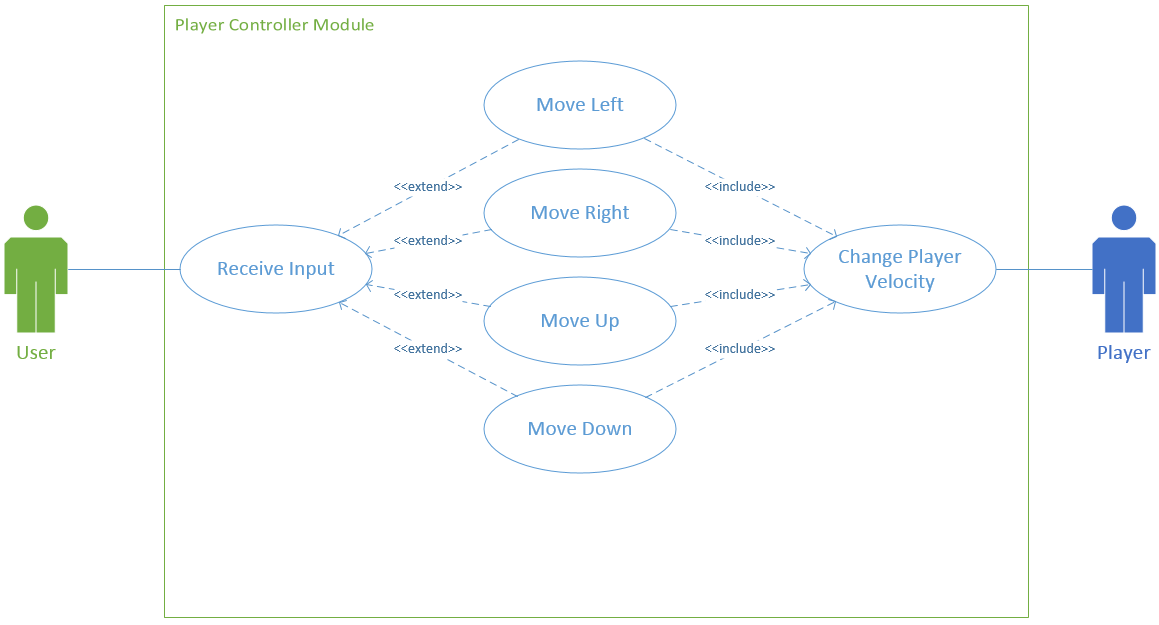
\includegraphics[scale=0.5]{images/Move.png}
		\caption{Move Player (UC-1)}
	\end{figure}
	\begin{figure}
		\centering
		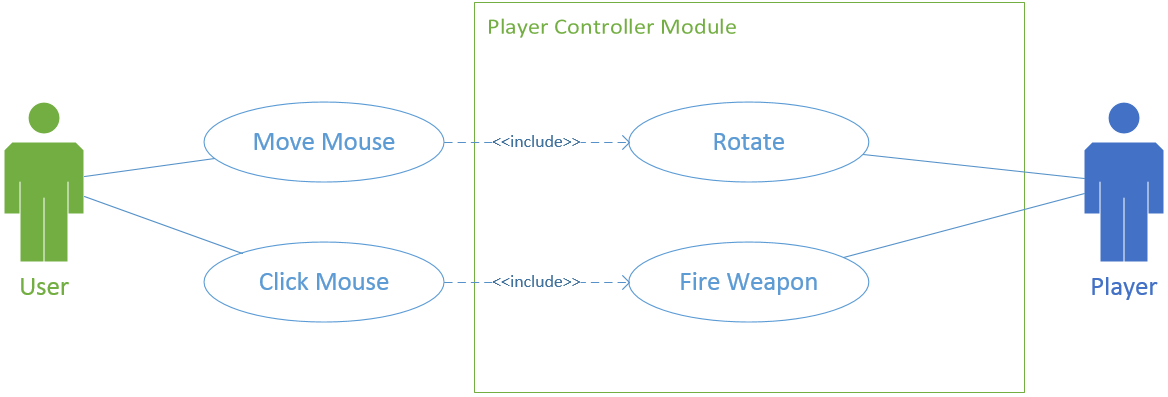
\includegraphics[scale=0.5]{images/FireWeapon.png}
		\caption{Fire Weapon (UC-2)}
	\end{figure}
	\begin{figure}
		\centering
		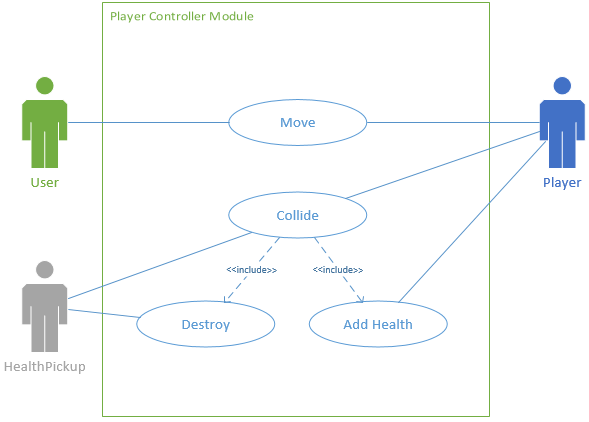
\includegraphics[scale=0.5]{images/CollectPickup.png}
		\caption{Collect Pickup (UC-3)}
	\end{figure}
	\begin{figure}
		\centering
		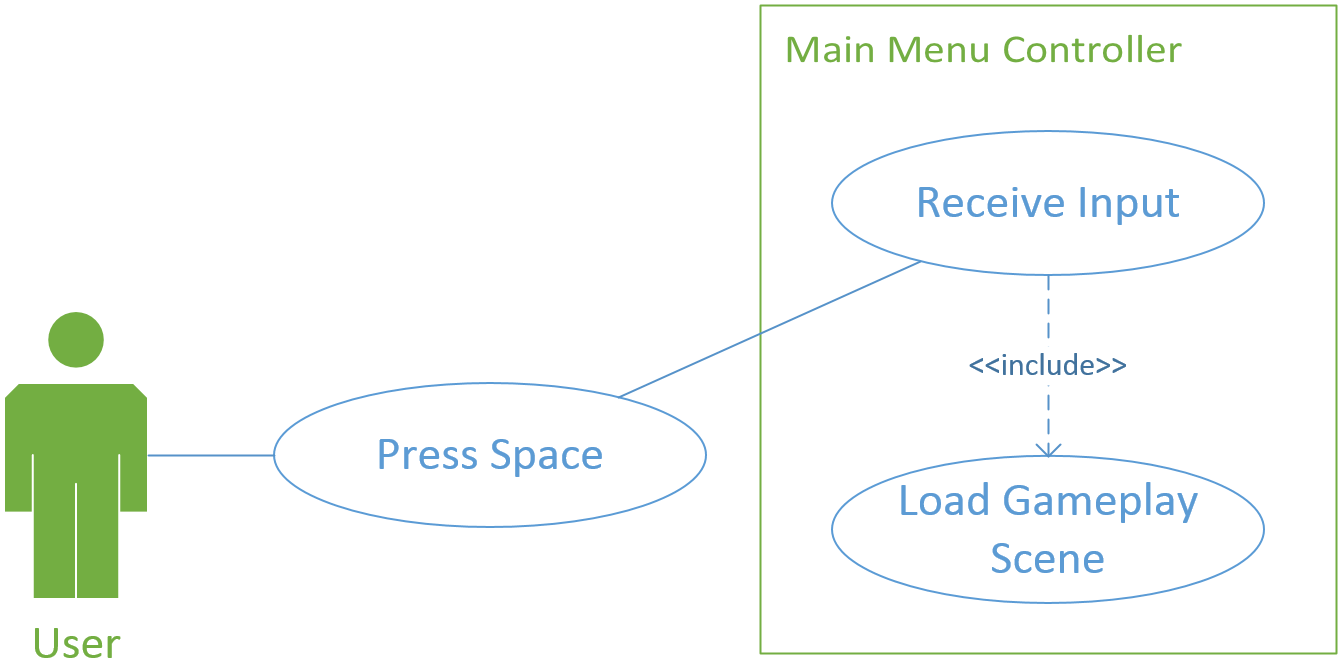
\includegraphics[scale=0.5]{images/BeginRound.png}
		\caption{Begin Round (UC-4)}
	\end{figure}
	\begin{figure}
		\centering
		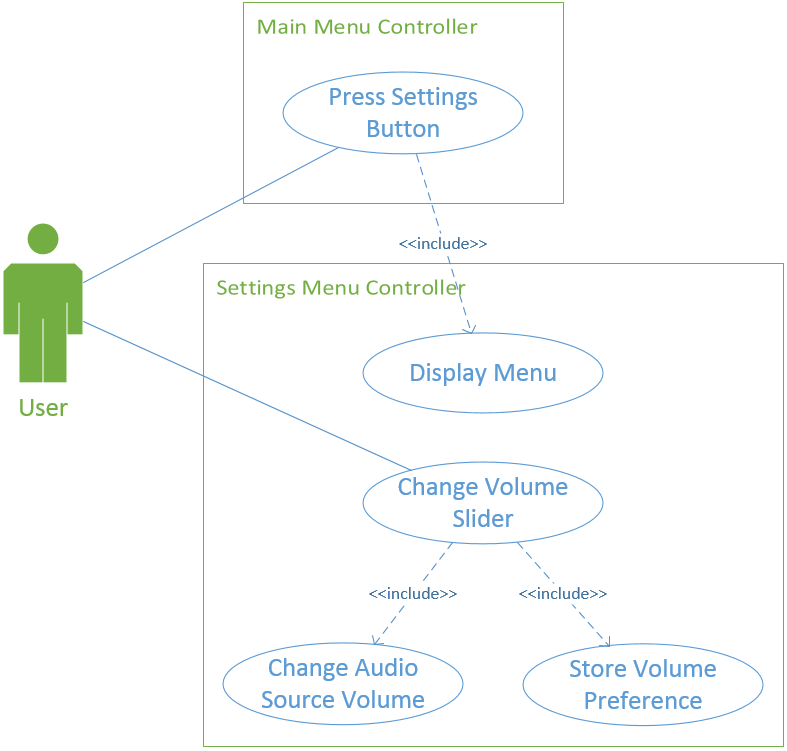
\includegraphics[scale=0.5]{images/ChangeSettings.png}
		\caption{Change Settings (UC-5)}
	\end{figure}
	\begin{figure}
		\centering
		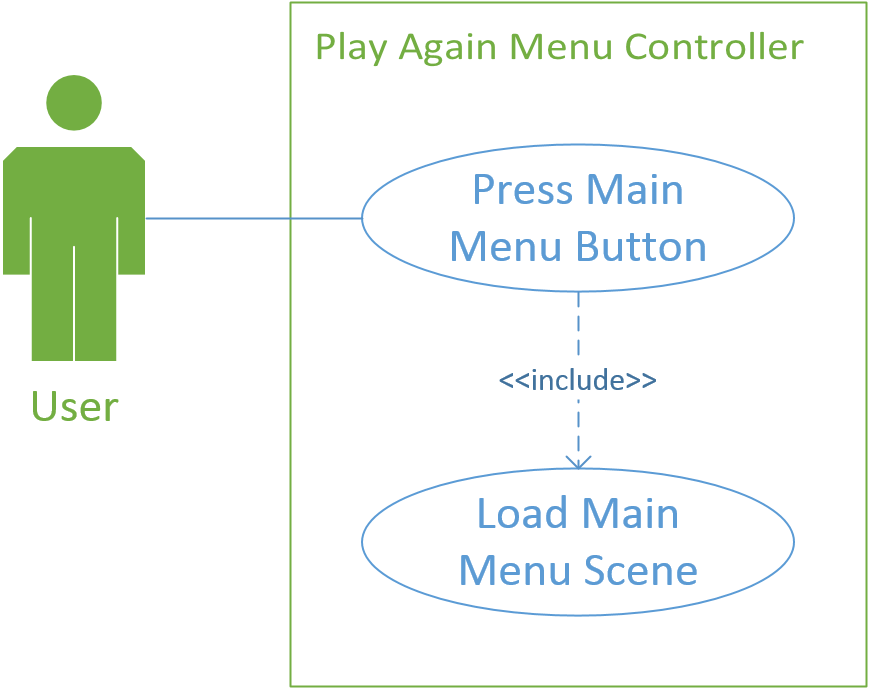
\includegraphics[scale=0.5]{images/ReturnToHome.png}
		\caption{Return to Main Menu (UC-6)}
	\end{figure}
	\begin{figure}
		\centering
		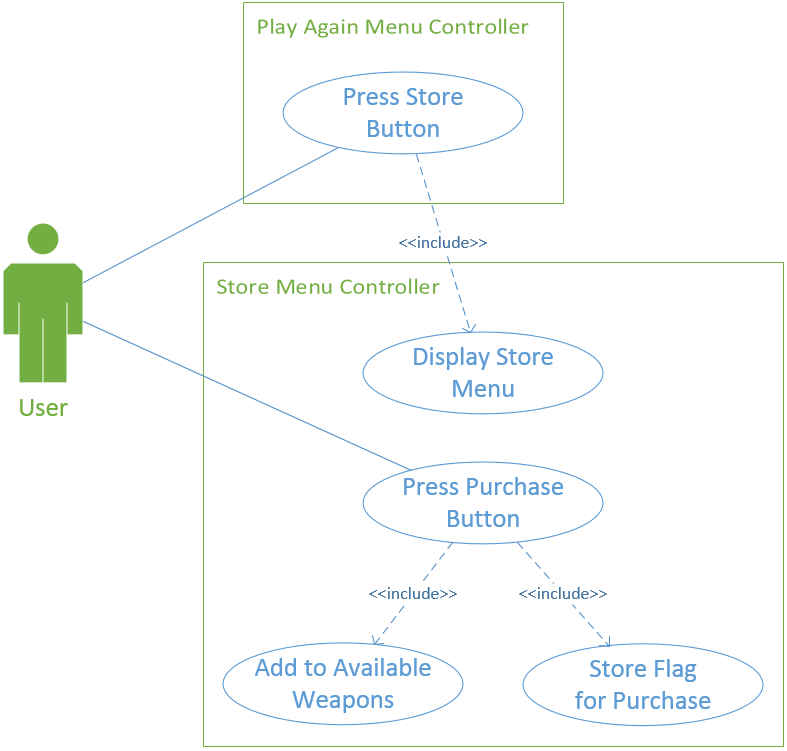
\includegraphics[scale=0.5]{images/PurchaseWeapon.png}
		\caption{Purchase Weapon (UC-7)}
	\end{figure}
	\begin{figure}
		\centering
		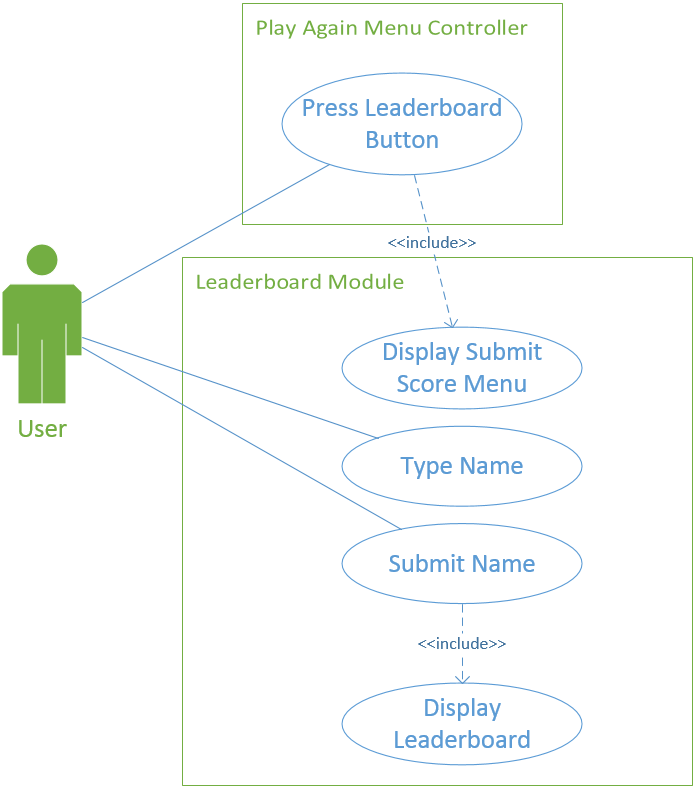
\includegraphics[scale=0.5]{images/SubmitScore.png}
		\caption{Submit Score to Leaderboard (UC-8)}
	\end{figure}
	\newpage
	\subsection{User Characteristics}
		Due to the nature of video games, there is a broad and diverse pool of potential users of The System. There is no reason to exclude individuals as potential users based on any age constraints ranging from children to the elderly. As such, no special knowledge or skills should be assumed for any user with the exception of the basic use of a computer, graphical user interfaces, and web browsers.
	\subsection{Constraints}
		\begin{reqlist}
			\item \textbf{Browser} \\
				Old or outdated browsers may not offer the proper support for prerequisite technologies such as WebGL and HTML5 to properly run The System. Given the variety of browsers that are either currently or previously available to the public, providing support for every version of every browser is simply not feasible.
			\item \textbf{Hardware} \\
				Much like the issues that can arise with antiquated browsers, older computers may not be able to meet the demands to adequately run The System due to hardware limitations.
			\item \textbf{Type of Device} \\
				With the proliferation of tablets and smartphones, many games being produced today are intended for these platforms. However, The System is designed with a more traditional set of mouse and keyboard controls. So although users may possibly be able to access and load The System via the browser on their smart device, there is currently no support for the touchscreen inputs used for these devices.
			\item \textbf{Internet Connection} \\
				Although The System itself does not depend on an internet connection or networking capabailities in any substantial way, some restrictions to the user's access to the internet may present constraints on The System as well. Most importantly, since The System is inherently web-based, the user will need some form of internet connection in order to access it. Additionally, the leaderboard feature present in the System will not be  able to submit or fetch scores to and from the database without a stable connection to the internet. However, the remainder of The System will still function correctly once loaded even without internet access.
		\end{reqlist}
	\subsection{Assumptions and Dependencies}
		\begin{reqlist}
			\item The user's browser is reasonably modern and able to adequately support contemporary software.
			\begin{reqlist}
				\item The browser was most recently updated within at least the last year.
				\item The browser offers support for HTML5/WebGL.
			\end{reqlist}
			\item The user is accessing The System on either a traditional desktop or laptop computer as opposed to a table or mobile device.
			\item The user's device consists of adequate hardware to adequately support contemporary software.
			\begin{reqlist}
				\item The device has a CPU containing at least 4 cores.
				\item The device has at least 4GB of RAM.
			\end{reqlist}
			\item The user has a stable enough connection to the internet to load The System within a reasonable amount of time, and preferably to submit and fetch leaderboard scores as well.
		\end{reqlist}

\section{User/Stakeholder Profiles}
\begin{center}
	\begin{tabular}{|c|c|c|} \hline
		\textbf{Stakeholder} & \textbf{Interests} & \textbf{Constraints} \\ \hline
		Player & Entertainment & Browser, Hardware, Device, and Connection limitations \\ \hline
		System Administrator & Maintenence & Maintains system hardware and databases \\ \hline
		Software Developer & Development & Runs in test environments \\ \hline
	\end{tabular}
\end{center}

\section{Core System Requirements}
	This section lists all of the core functional requirements for the System.
	\subsection{Storage Requirements}
		\begin{reqlist}
			\item The System shall not exceed a size of 20MB when exported by the Unity Game Engine.
			\item The System shall maintain all persistent data within a database of JSON objects handled by the IndexedDB API.
			\item The System shall not exceed 1MB of persistent data per browser.
		\end{reqlist}
	\subsection{Networking Requirements}
		\begin{reqlist}
			\item The System shall be hosted in a web-based environment.
			\item The System shall limit all network interactions to the use of an in-game leaderboard.
			\item The System shall notify the user of any inability to fetch or submit scores to the leaderboard.
			\item The System shall only attempt network interactions upon the user's request.
		\end{reqlist}
		
\section{Feature Requirements}
	This section lists all of the features to be implemented in the System.
	\subsection{General Features}
		\begin{reqlist}
			\item The System shall begin with a main menu screen.
			\begin{reqlist}
				\item The main menu shall include a title, a simple logo, and instructions for how to begin a round.
				\item The main menu shall allow the user to begin a round by pressing the space bar.
				\item The main menu shall give the user access to a settings menu by pressing a button in the bottom-right corner of the screen.
			\end{reqlist}
			\item The System shall allow the user to change selected game settings.
			\begin{reqlist}
				\item The settings menu shall allow the user to delete all persistent data stored by The System.
				\item The settings menu shall allow the user to set the volume of in-game music.
				\item The settings menu shall allow the user to set the volume of in-game sound effects.
				\item Volume shall be set on a scale of 0-1. For example, 0.5 would represent half the maximum volume.
				\item Any changes to the settings shall be persistent between sessions.
			\end{reqlist}
			\item The System shall include in-game currency.
			\begin{reqlist}
				\item The in-game currency shall made available for collection during each round of gameplay.
				\item The System shall treat in-game currency as a pickup.
				\item The amount of in-game currency collected shall be persistent between multiple sessions.
				\item The amount of in-game currency shall be erased upon the user pressing the ``delete data" button in the settings menu.
			\end{reqlist}
			\item The System shall include an in-game store allowing the user to purchase weapons and upgrades with in-game currency.
			\begin{reqlist}
				\item The store shall be accessible to the user after each round of gameplay.
				\item The store shall allow the user to make purchases by clicking a UI button.
				\item The store shall display the name, price, and description for each available item upon hovering over their purchase buttons.
				\item The store shall not allow the user to purchase an item already in their posession.
				\item The store purchases shall be persistent between multiple sessions.
				\item The store purchases shall be erased upon the user pressing the ``delete data" button in the settings menu.
			\end{reqlist}
			\item The System shall introduce a scoring system to rank players based on their performance for each round of gameplay.
			\begin{reqlist}
				\item The user's score shall be determined by the length of their round in hours, minutes, and seconds.
				\item The user's score shall be constantly visible during gameplay.
			\end{reqlist}
			\item The System shall contain a leaderboard interface which allows players to submit and compare their score with other users.
			\begin{reqlist}
				\item The leaderboard shall be hosted as a database on https://dreamlo.com/.
				\item The leaderboard shall be accessible to the user after each round of gameplay.
				\item The leaderboard shall display the 10 highest scores submitted.
				\item The leaderboard shall accept multiple scores from users submitting an existing name, keeping the highest score.
				\item The leaderboard shall not require the user to submit their score in order to view the top scores.
			\end{reqlist}
			\item The System shall dispaly a ``Game Over" screen upon the player exhausting all their lives.
			\begin{reqlist}
				\item The Game Over screen shall allow the player to return to the main menu, access the store, and submit their score to the leaderboard.
			\end{reqlist}
		\end{reqlist}
	\subsection{Gameplay Features}
		\begin{reqlist}
			\item The player shall be controlled via mouse and keyboard inputs from the user.
			\begin{reqlist}
				\item Pressing the directional keys during gameplay shall result in the player moving on screen in that direction.
				\item Moving the cursor on screen during gameplay shall result in the player rotating toward the direction of the cursor.
				\item Clicking the mouse or pressing the space bar during gameplay shall result in the player firing the current weapon in the direction the player is facing.
			\end{reqlist}
			\item The player will be provided with vitals which dictate their ability to survive and eliminate threats throughout a round.
			\begin{reqlist}
				\item The health vital shall determine how much damage the player can endure without losing a life.
				\item The default maximum health capacity shall be 100 units.
				\item The lives vital shall determine how many times the player can exhaust their full health before ending the round.
				\item The default maximum lives vital shall be 3 units.
				\item The energy vital shall determine how many times the player can fire a weapon before needing to recharge.
				\item The default maximum energy capacity shall be 100 units.
				\item The energy vital shall be increased by 2 units every second until reaching the maximum energy capacity.
				\item The vitals shall be constantly visible during gameplay.
			\end{reqlist}
			\item The System shall allow the player to select multiple different weapons during gameplay.
			\begin{reqlist}
				\item The System shall initially supply the user with a standard laser weapon.
				\item The System shall include a minimum of two alternative weapons in addition to the standard laser.
				\item The System shall make the additional weapons available in the in-game store.
			\end{reqlist}
			\item The System shall generate obstacles which damage the player upon impact.
			\begin{reqlist}
				\item The asteroid obstacle shall spawn at a random y-position offscreen.
				\item The asteroid obstacle shall travel at a fixed speed to the left side of the screen.
				\item The asteroid obstacle shall damage the player and enemies when it collides with them.
				\item The blackhole obstacle shall spawn at a random y-position offscreen.
				\item The blackhole obstacle shall travel at a fixed speed to the left side of the screen.
				\item The blackhole obstacle shall damage and destroy all other objects that collide with it.
			\end{reqlist}
			\item The System shall generate enemies which target the player to deal intentional damage.
			\begin{reqlist}
				\item The System shall generate two types of enemies designated "Type A Enemies" and "Type B Enemies"
				\item The system shalll spawn enemies at random locations off screen.
				\item Type B Enemies shall approach the Player from a distance until a suitable firing distance is achieved.
				\item Type B Enemies shall stay at a fixed position as long as they are within firing distance and shoot at the Player.
				\item Type B Enemies shall rotate to maintain a bearing on the Player.
				\item Type A Enemies shall approach the player from a distance until a suitable firing distance is achieved.
				\item Type A Enemies shall contrinue too follow the Player.
				\item Type A Enemies shall rotate to maintain a bearing on the player.
				\item Type A Enemies shall attempt to dodge the incoming laser fire from the player.
			\end{reqlist}
			\item The System shall generate pickups to aid the player in their survival.
			\begin{reqlist}
				\item Pickups shall be collected when the player collides with them in-game.
				\item Pickups shall have their colliders set as ``triggers" within the unity engine.
				\item The health pickup shall add 15 to the player's current health vital.
				\item The energy pickup shall add 15 to the player's current energy vital.
				\item The coin pickup shall add 10 to the user's available currency.
				\item Each pickup shall play a unique sound effect when collected.
			\end{reqlist}
			\item The System shall increase the difficulty of gameplay as the amount of time spent in a round progresses.
			\begin{reqlist}
				\item The progression of difficulty shall be managed by the Phase Manager module.
				\item The Phase Manager shall keep account of a set of phase multipliers for each enemy type and obstacle type.
				\item The Phase Manager shall increase these phase multipliers over time, switching between phases in 5 second intervals.
				\item The number of enemies generated shall increase as the phase multiplier value for each associated enemy increases.
				\item The time between each asteroid generation shall decrease by 20\% of the current asteroid phase multiplier value of the PhaseManager each asteroid phase with a floor of an asteroid generating every second.
			\end{reqlist}
			\item The System shall generate random events which introduce additional challenges to the player.
			\begin{reqlist}
				\item The events shall be managed by the Phase Manager module.
				\item The System shall evaluate whether an event should take place every 60 seconds.
				\item The event evaluation shall involve a 33\% chance that no event will occur.
				\item The events shall last 30 seconds.
				\item The duration of an event shall not count toward the time until the next event evaluation.
				\item The ``asteroid belt" event shall temporarily disable enemy generation and set the Obstacle Generator module to generate an asterod every 0.6 seconds.
				\item The ``nebula" event shall temporarily reduce the player's maximum energy capacity by half.
				\item The user shall be notified of an event taking place via a textual notification and sound effect.
			\end{reqlist}
		\end{reqlist}

%\section{UI Requirements}

\section{Performance Requirements}
	This sections lists all performance requirements laid out for the System.
	\subsection{Frame Rate Requirements}
	\begin{reqlist}
		\item The System shall at no time include spikes in frame rate that dip below 15 FPS.
		\item The System shall limit the number of average performance spikes to a maximum of 1 spike per second.
		\item The System shall limit the number of simultaneous Update() methods executing instructions every frame to a maximum of 10.
	\end{reqlist}

\section{Nonfunctional Requirements}
	This section lists the nonfunctional requirements pertaining to the System. 
	\subsection{Software-Related}
		\begin{reqlist}
			\item The System shall be developed using exclusively the C\# language.
			\item The System shall be designed using the Unity Game Engine.
			\item The System shall be exported to the WebGL platform using Unity's included build options.
		\end{reqlist}
	\subsection{Graphics \& Visuals}
		\begin{reqlist}
			\item The System shall use a native resolution of 1400x700 pixels.
			\item The System shall offer fullscreen support for a resolution of 1920x1080 pixels.
			\begin{reqlist}
				\item Any 16:9 aspect ratio display should also be supported as a result, at the possible expense of some minor graphical defects such as blurring at larger resolutions.
			\end{reqlist}
			\item The System shall only use the .png format for images.
			\item The System shall only use the .fbx format for 3D models.
		\end{reqlist}
	\subsection{Audio}
		\begin{reqlist}
			\item The System shall only use the .mp3, .ogg, and .wav formats for all music and sound effects.
			\item The System shall preload all audio assets prior to the beginning of gameplay.
			\item No audio files shall contain greater than 1 second of silence.
			\item No audio files used for music shall exceed 4 minutes in length.
			\item No audio files used for music shall exceed 9MB in size.
			\item No audio files used for sound effects shall exceed 4 seconds in length.
			\item No audio files used for sound effects shall exceed 1.5MB in size.
			\item Audio files shall be compressed during gameplay to minimize loadtimes.
		\end{reqlist}

\newpage
\section{Requirements Traceability Matrix}
	\begin{figure}[!htb]
		\centering
		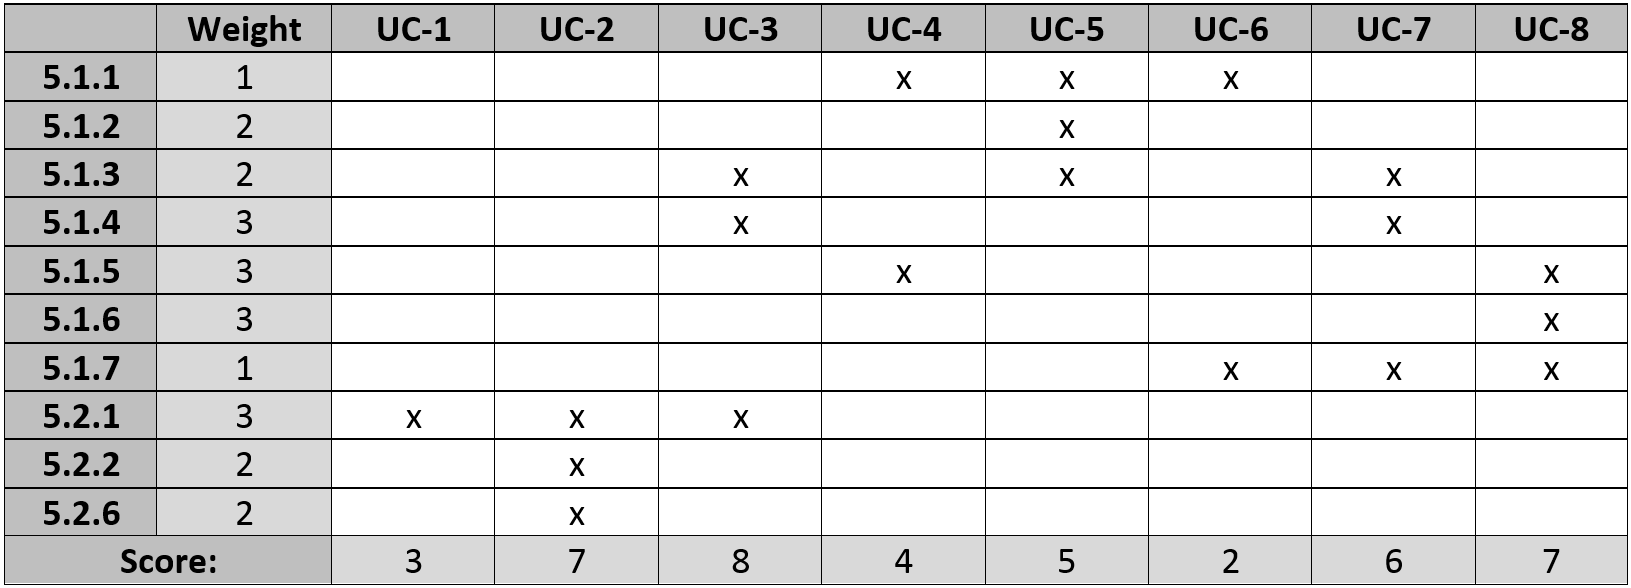
\includegraphics[scale=0.35]{images/Matrix.png}
		\caption{A requirements traceability matrix for the major use cases of The System.}
	\end{figure}
\listoffigures
\end{document}